\subsection{Trading Intensity} \label{sec:A8}
The extraordinary performance of our proposed LLM-based methodology warrants a careful examination of its implementation costs and practical viability. While our primary objective has been to develop a framework that better captures the economic content of news articles and their subsequent market impact, the practical implementation of such strategies necessarily involves trading frictions that could affect their real-world efficacy. In this section, we analyze the trading intensity patterns of both methodologies to provide a more complete assessment of their relative merits and to understand how transaction costs might influence their comparative advantages.
We begin by examining the temporal evolution of open positions for both approaches, which provides insights into their underlying trading dynamics and stability characteristics. This analysis is followed by detailed trading intensity metrics and concludes with a reassessment of portfolio statistics after accounting for transaction costs.

%----------------------------------------------------
\inserthere{fig:open_positions_comparison}

\begin{figure}[htbp]
\caption{Evolution of Open Positions: KMeans vs LLM Clustering}
\label{fig:open_positions_comparison}

% Panel A: KMeans
\begin{subfigure}{\textwidth}
\caption{Panel A: KMeans Clustering}
\centering
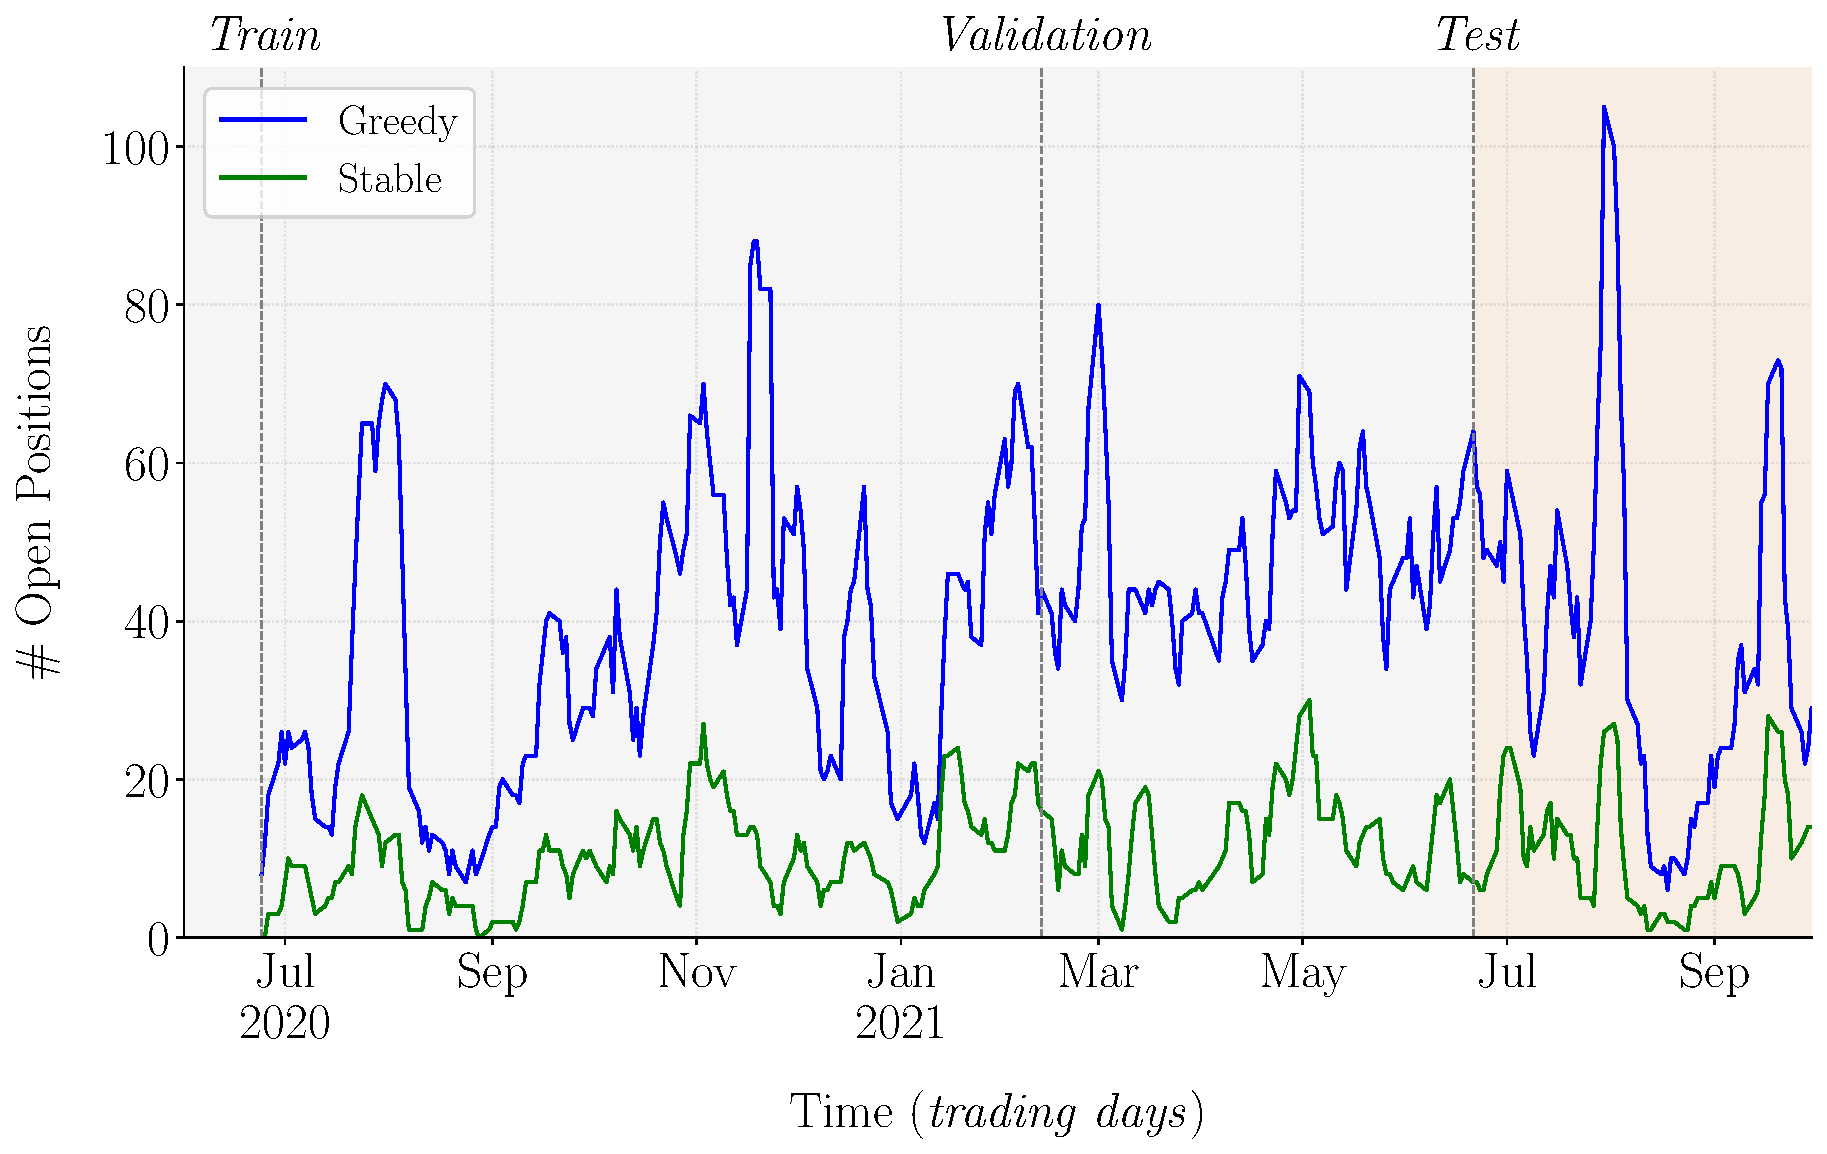
\includegraphics[scale=0.45]{fig_A6a_KMeans_Open_Positions.pdf}
\end{subfigure}

\vspace{0.7cm}

% Panel B: LLM
\begin{subfigure}{\textwidth}
\caption{Panel B: LLM Clustering}
\centering
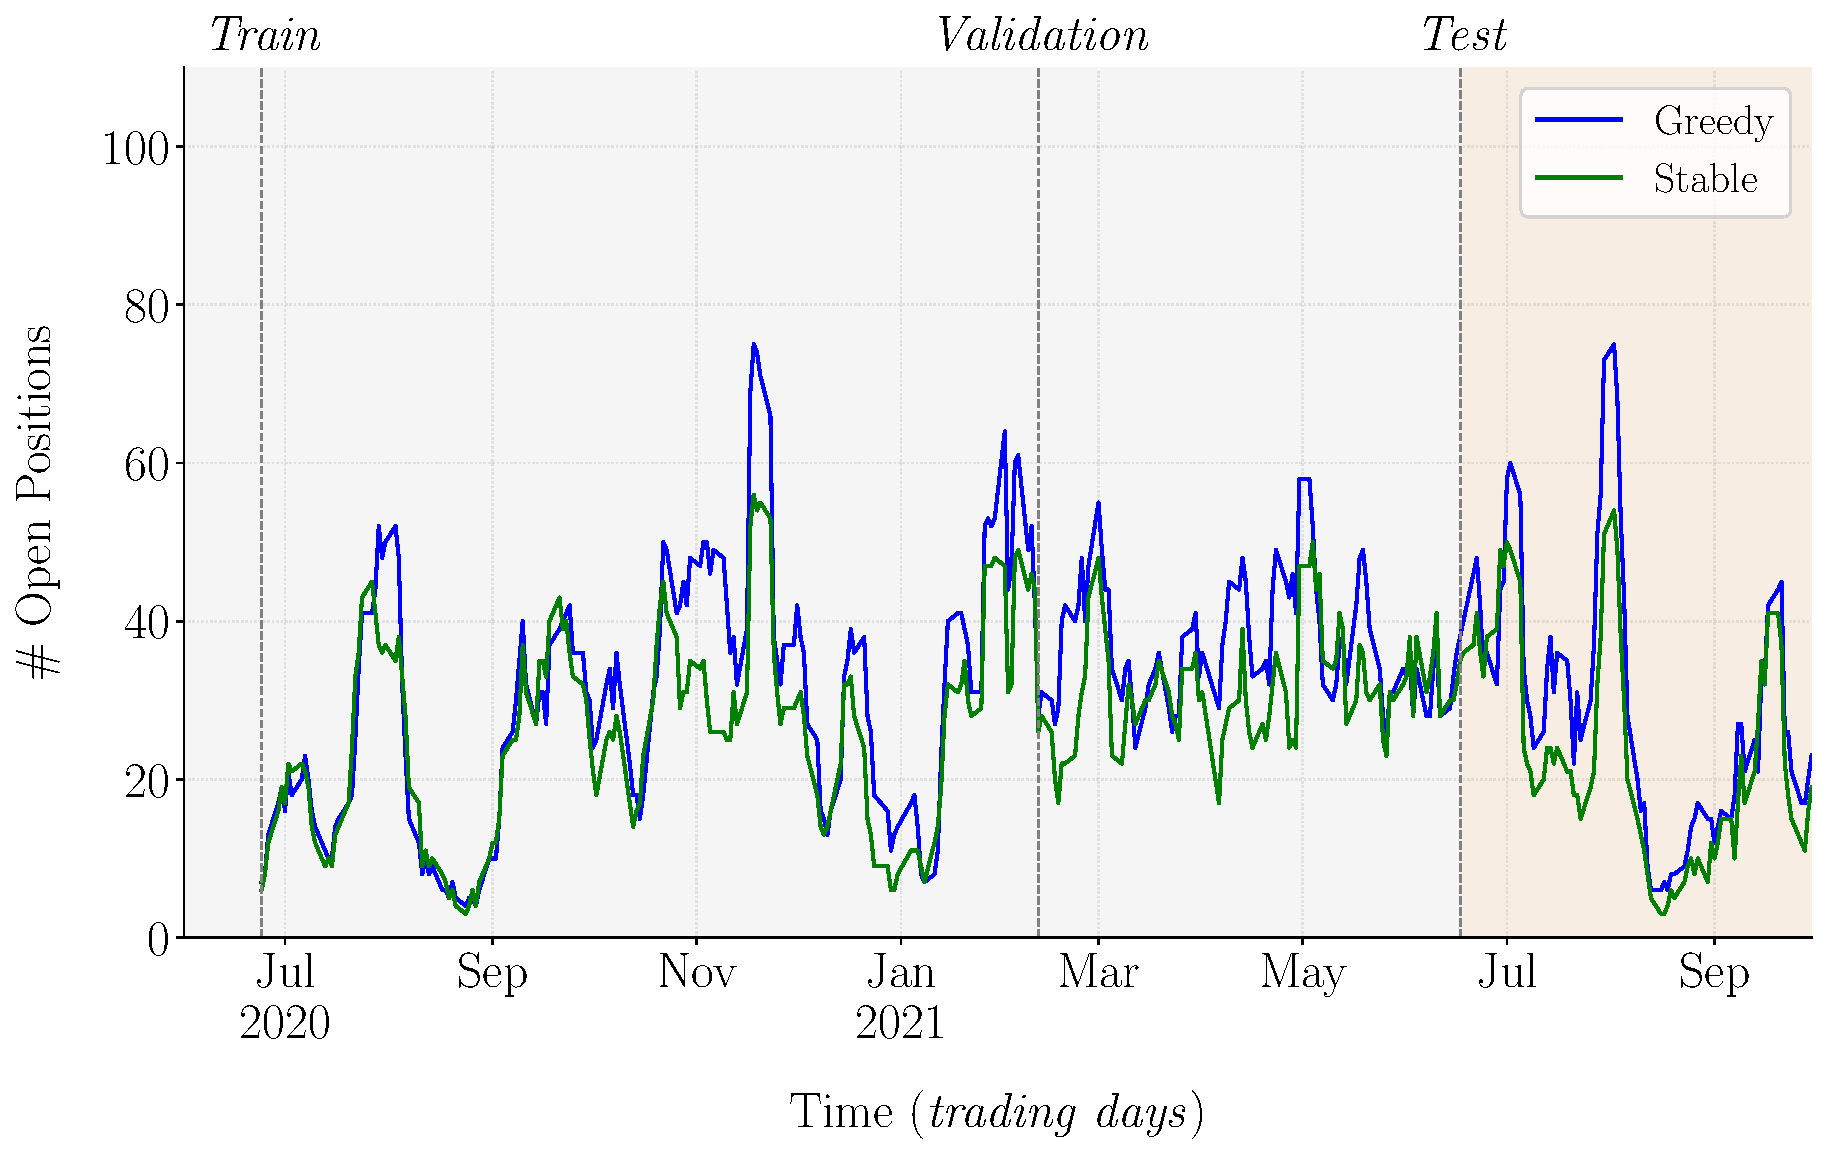
\includegraphics[scale=0.45]{fig_A6b_LLAMA_Open_Positions.pdf}
\end{subfigure}

\vspace{0.2cm}
\begin{minipage}{\textwidth}
\setlength{\parindent}{0pt}
{\footnotesize\textit{Note: 
This figure shows the daily evolution of the number of open positions for both Greedy (blue) and Stable (green) algorithms across different data splits (Train, Validation, Test) using KMeans clustering (Panel A) and LLM clustering (Panel B). The time period spans from July 2020 to September 2021. Vertical dashed lines separate the different data splits. The Greedy algorithm selects clusters that maximize (minimize) the cluster-average-$SR$ for long (short) positions, while the Stable algorithm minimizes the rank difference between training and validation rankings. The number of traded clusters is $\theta = 0.5k=13$ for KMeans ($k^*=26$ clusters) and $\theta = 0.5k=10$ for LLM ($k^*=20$ clusters).
}}
\end{minipage}
\end{figure}
%----------------------------------------------------

% < Reference to: \cref{fig:open_positions_comparison} >
The temporal evolution of open positions, as illustrated in \cref{fig:open_positions_comparison},  reveals fundamental differences in the stability and reliability of trading signals generated by KMeans versus LLM-based clustering approaches. The KMeans implementation exhibits pronounced volatility in position management, particularly evident in the Greedy algorithm's behavior, which shows extreme fluctuations ranging from 6 to 105 positions. This erratic pattern suggests that KMeans-detected clusters are highly sensitive to market noise and potentially capture transient correlations rather than fundamental relationships. The substantial divergence between Greedy and Stable algorithms under KMeans further underscores the method's instability, as even minor variations in cluster selection criteria lead to dramatically different trading decisions.
%
In stark contrast, the LLM-based approach demonstrates remarkably more coherent and stable position management. Both Greedy and Stable algorithms maintain more closely aligned position counts, typically ranging between 20 and 75 positions, with highly correlated temporal movements. This convergence in behavior between algorithms suggests that LLM-identified clusters capture more fundamental and persistent market relationships. Particularly telling is the test period performance, where KMeans exhibits increased position volatility and extreme spikes, while the LLM approach maintains consistent position patterns across both algorithms. This stability in the out-of-sample period provides strong evidence that LLM-derived signals, grounded in economic analysis of firm-specific shocks, generalize more effectively to unseen data.

%----------------------------------------------------
\inserthere{tab:trading_intensity_comparison}

\begin{table}[htbp] 
\caption{Trading Intensity Analysis: Model Comparison} 
\centering 
\label{tab:trading_intensity_comparison}

\begin{subtable}{\textwidth}
\caption{Panel A: KMeans}
\centering 
{\small
\begin{tabular}{lcccccccccc}
\toprule
\textbf{Split} & \textbf{Algorithm} & \multicolumn{4}{c}{\textbf{\# Open Positions}} & \multicolumn{2}{c}{\textbf{Trading Activity (\%)}} & \multicolumn{2}{c}{\textbf{Trading Costs (\%)}} \\
\cmidrule(lr{0.6em}){3-6} \cmidrule(lr{0.6em}){7-8} \cmidrule(lr{0.6em}){9-10}
& & \textbf{Avg}. & \textbf{Std}. & \textbf{Max} & \textbf{Min} & \textbf{Turnover} & \textbf{Changes/Pos.} & \textbf{Cost} & \textbf{Active} \\
\midrule
\multirow{2}{*}{All} & \textit{Greedy} & 40.1 & 18.59 & 105 & 6 & 32.03 & 0.798 & 0.0961 & 100.0 \\
 & \textit{Stable} & 10.77 & 6.41 & 30 & 0 & 34.75 & 3.228 & 0.1042 & 99.1 \\
\midrule
\multirow{2}{*}{Train} & \textit{Greedy} & 36.4 & 19.33 & 88 & 7 & 30.59 & 0.840 & 0.0918 & 100.0 \\
 & \textit{Stable} & 9.89 & 5.93 & 27 & 0 & 33.73 & 3.412 & 0.1012 & 98.2 \\
\midrule
\multirow{2}{*}{Validation} & \textit{Greedy} & 48.4 & 10.00 & 80 & 30 & 31.39 & 0.649 & 0.0942 & 100.0 \\
 & \textit{Stable} & 12.34 & 6.05 & 30 & 1 & 33.42 & 2.708 & 0.1003 & 100.0 \\
\midrule
\multirow{2}{*}{Test} & \textit{Greedy} & 38.8 & 21.74 & 105 & 6 & 35.86 & 0.925 & 0.1076 & 100.0 \\
 & \textit{Stable} & 10.84 & 7.47 & 28 & 1 & 39.30 & 3.626 & 0.1179 & 100.0 \\
\bottomrule
\end{tabular}
}
\end{subtable}

\vspace{0.6cm}

\begin{subtable}{\textwidth}
\caption{Panel B: LLM}
\centering
{\small
\begin{tabular}{lcccccccccc}
\toprule
\textbf{Split} & \textbf{Algorithm} & \multicolumn{4}{c}{\textbf{\# Open Positions}} & \multicolumn{2}{c}{\textbf{Trading Activity (\%)}} & \multicolumn{2}{c}{\textbf{Trading Costs (\%)}} \\
\cmidrule(lr{0.6em}){3-6} \cmidrule(lr{0.6em}){7-8} \cmidrule(lr{0.6em}){9-10}
& & \textbf{Avg}. & \textbf{Std}. & \textbf{Max} & \textbf{Min} & \textbf{Turnover} & \textbf{Changes/Pos.} & \textbf{Cost} & \textbf{Active} \\
\midrule
\multirow{2}{*}{All} & \textit{Greedy} & 31.8 & 14.84 & 75 & 4 & 39.21 & 1.234 & 0.1176 & 100.0 \\
 & \textit{Stable} & 26.61 & 12.16 & 56 & 3 & 39.18 & 1.473 & 0.1175 & 100.0 \\
\midrule
\multirow{2}{*}{Train} & \textit{Greedy} & 29.9 & 16.34 & 75 & 4 & 40.42 & 1.351 & 0.1212 & 100.0 \\
 & \textit{Stable} & 25.54 & 12.90 & 56 & 3 & 40.45 & 1.584 & 0.1213 & 100.0 \\
\midrule
\multirow{2}{*}{Validation} & \textit{Greedy} & 37.0 & 7.69 & 58 & 24 & 38.43 & 1.039 & 0.1153 & 100.0 \\
 & \textit{Stable} & 31.38 & 6.82 & 50 & 17 & 37.95 & 1.209 & 0.1138 & 100.0 \\
\midrule
\multirow{2}{*}{Test} & \textit{Greedy} & 29.7 & 16.24 & 75 & 6 & 37.56 & 1.264 & 0.1127 & 100.0 \\
 & \textit{Stable} & 23.43 & 13.71 & 54 & 3 & 37.85 & 1.615 & 0.1135 & 100.0 \\
\bottomrule
\end{tabular}
}
\end{subtable}

\vspace{0.5cm}
\begin{minipage}{\textwidth}
\setlength{\parindent}{0pt}
\small\textit{Note: 
This table presents trading intensity metrics for both Greedy and Stable algorithms across different data splits for two different models: KMeans (Panel A) and LLM (Panel B). 
The metrics are computed at a daily frequency. The `\# Open Positions' columns report position-related statistics: 
`Avg.' shows the mean number of concurrent open positions per day, `Std.' represents their standard deviation, while 
`Max' and `Min' indicate the maximum and minimum number of positions held simultaneously. Under `Trading Activity (\%)', 
`Turnover' is calculated as the sum of absolute changes in position sizes divided by the total portfolio size, expressed 
as a percentage; formally, $Turnover_t = 100 \times (\sum_i |w_{i,t} - w_{i,t-1}|)/(\sum_i |w_{i,t}|)$, where $w_{i,t}$ 
represents the position size in asset $i$ at time $t$. `Changes/Pos.' represents the average number of modifications per 
position per day, computed as the daily turnover divided by the average number of positions, providing insight into how 
actively individual positions are managed. 
The `Trading Costs (\%)' section reports `Cost' as the average daily implementation shortfall (computed as the product of daily turnover and a conservative transaction cost parameter of 30 basis points, representing both direct and indirect trading costs) expressed in percentage terms, while `Active' shows the percentage of trading days with at least one open position.
%
%The `Trading Costs (\%)' section reports `Cost' as the average daily implementation 
%shortfall (computed as the difference between gross and net returns) expressed in percentage terms, while `Active' shows 
%the percentage of trading days with at least one open position. 
All metrics are first computed daily and then averaged over their respective periods, except for Max and Min positions which represent the absolute extremes over each period.
}
\end{minipage}
\end{table}
%----------------------------------------------------

% < Reference to: \cref{tab:trading_intensity_comparison} >
The trading intensity metrics, detailed in \cref{tab:trading_intensity_comparison}, provide quantitative validation of the structural differences between KMeans and LLM clustering approaches. Under KMeans, the dramatic disparity between Greedy and Stable algorithms (averaging 40.1 versus 10.77 positions, with standard deviations of 18.59 and 6.41 respectively) reflects the method's fundamental instability. More concerning is the Stable algorithm's exceptionally high Changes/Position ratio (3.228 versus 0.798 for Greedy), indicating frequent position adjustments necessitated by the transient nature of KMeans-identified clusters.
The LLM implementation demonstrates substantially more balanced and stable metrics across both algorithms. Average position counts converge (31.8 for Greedy, 26.61 for Stable) with more moderate standard deviations (14.84 and 12.16), suggesting that both aggressive and conservative cluster selection approaches identify similar, fundamentally-driven trading opportunities. The more balanced Changes/Position ratios (1.234 and 1.473) and consistent turnover rates (approximately 39\% for both algorithms) indicate that LLM-identified clusters require less frequent rebalancing, supporting the hypothesis that they capture more persistent market relationships.
These patterns become particularly pronounced in the test period, where KMeans shows increased turnover (reaching 39.30\% for Stable) and position volatility, while the LLM approach maintains more stable trading activity (37.56\% and 37.85\% turnover for Greedy and Stable). This superior out-of-sample stability provides compelling evidence that LLM's economic approach to cluster identification produces more robust and generalizable trading signals compared to the purely statistical approach of KMeans.

%----------------------------------------------------
\inserthere{tab:portfolio_statistics_comparison_net}

\begin{table}[H] 
\caption{Portfolio Statistics Comparison: KMeans vs LLM Clustering (net of Trading Costs)} 
\centering
\label{tab:portfolio_statistics_comparison_net}

\renewcommand{\arraystretch}{1.1}
\newcolumntype{P}[1]{>{\centering\arraybackslash}p{#1}}

% Panel A: KMeans
\begin{subtable}{\textwidth}
\caption{Panel A: Statistics of $\mathcal{P}_{\text{KMeans}}$}
\centering
{\small
\begin{tabular}{
 P{1.28cm} P{0.9cm} P{0.9cm} P{0.9cm} P{0.9cm} P{0.9cm} P{0.9cm} 
 P{0.9cm} P{1cm} P{0.9cm} P{0.9cm} P{0.9cm} P{0.9cm}
}
\Xhline{2\arrayrulewidth}
\textbf{Split} & \textbf{Algo.} & \textbf{Cum. Ret.} & \textbf{Avg. Ret.} & \textbf{St. Dev.} & \textbf{Sharpe Ratio} & \textbf{Sortino Ratio} & \textbf{Max. DD} & \textbf{Calmar Ratio} & \textbf{Skew.} & \textbf{Exc. Kurt.} & \textbf{VaR 95\%} & \textbf{CVaR 95\%} \\
\Xhline{2\arrayrulewidth}
\multirow{2}{*}{All} & \textit{Greedy} & 0.780 & -17.3 & 9.6 & -2.0 & -1.7 & -24.7 & -0.7 & -0.48 & 3.90 & -14.0 & -24.2 \\
 & \textit{Stable} & 1.058 & 4.4 & 17.0 & 0.3 & 0.3 & -14.2 & 0.3 & 0.15 & 5.01 & -24.5 & -38.3 \\
\hline
\multirow{2}{*}{Train} & \textit{Greedy} & 0.823 & -25.6 & 11.6 & -2.5 & -2.0 & -18.2 & -1.4 & -0.51 & 2.71 & -19.4 & -29.9 \\
 & \textit{Stable} & 1.057 & 8.7 & 19.9 & 0.4 & 0.4 & -14.2 & 0.6 & -0.25 & 3.21 & -31.9 & -46.0 \\
\hline
\multirow{2}{*}{Validation} & \textit{Greedy} & 1.000 & -0.0 & 7.5 & -0.0 & -0.0 & -5.8 & -0.0 & -0.50 & 0.95 & -12.1 & -17.9 \\
 & \textit{Stable} & 1.050 & 14.7 & 13.4 & 1.0 & 1.0 & -5.3 & 2.8 & -0.27 & 1.99 & -20.6 & -30.9 \\
\hline
\multirow{2}{*}{Test} & \textit{Greedy} & 0.937 & -20.0 & 6.6 & -3.4 & -3.5 & -9.1 & -2.2 & 1.55 & 4.31 & -8.9 & -12.0 \\
 & \textit{Stable} & 0.924 & -23.6 & 14.2 & -1.9 & -2.0 & -10.0 & -2.4 & 2.48 & 14.59 & -20.6 & -28.5 \\
\Xhline{2\arrayrulewidth}
\end{tabular}
}
\end{subtable}

\vspace{0.5cm}

% Panel B: LLM
\begin{subtable}{\textwidth}
\caption{Panel B: Statistics of $\mathcal{P}_{\text{LLM}}$}
\centering
{\small
\begin{tabular}{
 P{1.28cm} P{0.9cm} P{0.9cm} P{0.9cm} P{0.9cm} P{0.9cm} P{0.9cm} 
 P{0.9cm} P{1cm} P{0.9cm} P{0.9cm} P{0.9cm} P{0.9cm}
}
\Xhline{2\arrayrulewidth}
\textbf{Split} & \textbf{Algo.} & \textbf{Cum. Ret.} & \textbf{Avg. Ret.} & \textbf{St. Dev.} & \textbf{Sharpe Ratio} & \textbf{Sortino Ratio} & \textbf{Max. DD} & \textbf{Calmar Ratio} & \textbf{Skew.} & \textbf{Exc. Kurt.} & \textbf{VaR 95\%} & \textbf{CVaR 95\%} \\
\Xhline{2\arrayrulewidth}
\multirow{2}{*}{All} & \textit{Greedy} & 0.891 & -8.5 & 9.7 & -0.9 & -1.0 & -12.3 & -0.7 & 1.44 & 9.81 & -15.7 & -21.2 \\
 & \textit{Stable} & 0.928 & -5.6 & 8.6 & -0.7 & -0.7 & -11.7 & -0.5 & 0.31 & 2.18 & -12.9 & -18.7 \\
\hline
\multirow{2}{*}{Train} & \textit{Greedy} & 0.910 & -13.4 & 11.5 & -1.2 & -1.3 & -12.3 & -1.1 & 1.63 & 8.83 & -19.4 & -23.2 \\
 & \textit{Stable} & 0.964 & -5.5 & 10.0 & -0.6 & -0.6 & -9.7 & -0.6 & 0.21 & 1.60 & -14.8 & -21.6 \\
\hline
\multirow{2}{*}{Validation} & \textit{Greedy} & 0.985 & -4.3 & 8.1 & -0.5 & -0.6 & -4.3 & -1.0 & 0.19 & 1.17 & -11.6 & -18.0 \\
 & \textit{Stable} & 0.947 & -14.3 & 7.0 & -2.2 & -2.0 & -6.1 & -2.4 & 0.17 & 1.17 & -13.0 & -16.5 \\
\hline
\multirow{2}{*}{Test} & \textit{Greedy} & 0.995 & -1.5 & 6.2 & -0.2 & -0.3 & -1.9 & -0.8 & 1.02 & 6.91 & -8.2 & -12.1 \\
 & \textit{Stable} & 1.009 & 3.1 & 7.0 & 0.4 & 0.5 & -1.8 & 1.7 & 0.91 & 1.98 & -10.8 & -12.4 \\
\Xhline{2\arrayrulewidth}
\end{tabular}
}
\end{subtable}

\vspace{0.5cm}
\begin{minipage}{\textwidth}
\setlength{\parindent}{0pt}
{\small\textit{Note:
Portfolio statistics of trading strategies based on clusters obtained from KMeans (Panel A) and LLM (Panel B) approaches.
The statistics provided include performance metrics (Cumulative Return, Average Return (\%)), risk measures (Standard Deviation (\%), Maximum Drawdown (\%), Value at Risk (\%), Conditional Value at Risk (\%)), risk-adjusted performance ratios (Sharpe Ratio, Sortino Ratio, Calmar Ratio), and return distribution characteristics (Skewness, Excess Kurtosis). These statistics are provided for both cluster-selection algorithms: Greedy and Stable.
Except for the Cumulative Return, all returns are annualized. The Sharpe Ratio is computed using the daily returns, assuming 252 trading days in a year. The Sortino Ratio is calculated using the daily downside returns. The Maximum Drawdown is the maximum loss from a peak to a trough. The Calmar Ratio is the ratio of the annualized return to the maximum drawdown. Skewness measures the asymmetry of the return distribution, while Kurtosis quantifies the tails' thickness. The Value at Risk (VaR) and Conditional Value at Risk (CVaR) are calculated at a 95\% confidence level.
%
All returns are calculated net of transaction costs. We implement a conservative transaction cost estimate of 30 basis points (0.30\%) per trade, which accounts for both direct costs (commissions, fees) and indirect costs (bid-ask spreads, market impact). 
%Transaction costs for each day are computed as the product of daily portfolio turnover and the transaction cost parameter ($TC = \text{turnover} \times 0.30\%$). Daily turnover is measured as the ratio of the absolute change in positions to the total portfolio size: $\text{Turnover} = \sum|Position_{t} - Position_{t-1}| / \sum|Position_{t}|$. This implementation follows standard practice in the literature (see, e.g., \citet{frazzini2012}) and provides a realistic assessment of strategy profitability in real market conditions.
%
The Greedy algorithm longs (shorts) clusters that maximize (minimize) the cluster-average-$SR$ in the validation sample subject to a positivity (negativity) constraint, while the Stable algorithm longs (shorts) clusters that minimize the rank difference between the training and validation rankings of the cluster-average-$SR$'s subject to a positivity (negativity) constraint, which is now imposed on both sample splits. In both algorithms, the cardinality of each leg is upper-bounded by a hyperparameter $\theta$.
The holding period of the beta-neutral positions is set to $L$ = 4 trading days for both approaches. The number of traded clusters is $\theta = 0.5k=13$ for KMeans ($k^*=26$ clusters) and $\theta = 0.5k=10$ for LLM ($k^*=20$ clusters). The selection criteria for these hyperparameters ($L,\theta$) is based on maximizing the Sharpe Ratios of the train and validation samples.
}}
\end{minipage}
\end{table}
%----------------------------------------------------
% < Reference to: tab:portfolio_statistics_comparison_net >
Finally, the introduction of trading costs significantly impacts the performance metrics of both clustering approaches (see \cref{tab:portfolio_statistics_comparison_net}), though with notably different implications for their practical viability. The KMeans-based strategy exhibits substantial performance degradation, particularly evident in the test period where both algorithms generate significant losses (Greedy: -20.0\%, Stable: -23.6\% average annual returns). This deterioration is accompanied by elevated risk metrics, with the Stable algorithm showing particularly concerning characteristics including high standard deviation (14.2\%) and extreme kurtosis (14.59) in the test period, suggesting frequent occurrence of extreme returns.
In contrast, the LLM-based approach demonstrates superior resilience to trading costs, maintaining more stable performance characteristics across all periods. Most notably, in the test period, the strategy achieves near-neutral to positive performance (Greedy: -1.5\%, Stable: +3.1\% annual returns) with substantially lower risk metrics (standard deviations of 6.2\% and 7.0\% respectively). The LLM approach's more moderate VaR and CVaR measures (around -8.2\% to -12.4\% in the test period) compared to KMeans (-8.9\% to -28.5\%) further underscore its superior risk management characteristics under transaction costs.
This stark contrast in net performance can be attributed to the fundamentally different nature of the signals generated by each approach. While KMeans' statistically-driven clusters require frequent rebalancing that amplifies transaction costs, the LLM's economically-motivated clusters appear to identify more persistent price patterns that remain profitable even after accounting for trading frictions. However, it is worth noting that neither approach was explicitly optimized for transaction cost efficiency, suggesting potential for further improvement through cost-aware portfolio construction. These results highlight that while our LLM-based news parser successfully captures predictable market reactions to news articles, practitioners implementing such strategies would benefit from incorporating transaction costs into their optimization framework.
